
\chapter{Auditory Memory Mosaicing}

\minitoc

\section{Abstract}

Memory Mosaicing is a real-time sonic collage experience employing a perceptually-motivated model for representating and attending to sounds. This model relates the ongoing auditory world to previously learned ``sonic memories''.  Using a mobile platform, a user of the system wears earphones listening to an augmented sonic world which relates the incoming microphone stream to previously segmented sound clips, or sonic memories, creating a ongoing mosaic of sonic memories.  The system starts with an empty knowledge-base of sounds and continually stores only the segments of sounds which are determined salient and unclassified by a machine listening model.  The engine for synthesis is concatenative, matching the incoming segments to the learned ''sonic memories''.  The experience works in real-time on an iPhone 3 and above and has interactive parameters controlling the synthesis engine as well as the ability to learn from the user's own music library.  The experience of the iPhone app is multi-fold, creating a novel platform for investigating the role of memory in perception or as compositional or performance tool which grows its own expressive capabilities the more it hears.

\section{Introduction}

The juxtaposition of fragments of sound as an arts practice has roots at least as early as music concrete, a compositional technique assembling various natural found sounds in order to produce a collage of sound.  Digital Sampling came in the 1970's allowing sound segments to be triggered using an interface such as a keyboard or pad.  More recent techniques have focused on corpus-based concatenative synthesis, where a target sound is matched to a stored database of segments or sounds (for a comprehensive review, see \cite{Schwarz2006}).  

This chapter focuses on describing practical outputs in developing auditory scene synthesis.  The culmination of this practice will lead to the development of an application, ``Memory Mosaic'', which delivers an automated sonic-collage to a single user wearing headphones.  This application will also later be used in combination with the developments in my visual-practice in Chapter 7.   Before developing this application, however, I will discuss a few outputs created along the way which focused on exploring the use of spatialization, cut-up, narrative, and memory within a sonic collage practice.  

\section{Sonic Graffiti}

The first practical output I developed towards building an auditory scene synthesis is an application called ``Sonic Graffiti''.  The aim of this application was to create a soundscape based on a collage of sounds that had been recorded at different locations in 3-dimensional space.  A participant of the application could record sounds whenever they pressed a button and could do so in different locations in 3-dimensional space.  Then, when the participant would move in space, they would be able to hear the sounds they recorded as a continuous loop coming from the original location that they were recorded.  The interest in developing this application was (1) to synthesize an acoustic scene by replaying sound fragments based on their original location in space, and (2) to discover more about 3-dimensional sound perception.  My target platform at the time of development was the Apple iPhone 4, which includes a GPS sensor, digital compass, microphone, and audio output.  To begin with, I needed to discover how to record a set of sounds that could be re-positioned based on how a user moved around in 3-dimensional space.

\subsection{Methods}

\subsubsection{3-dimensional Sound Perception}\label{sec:binauralization}
To recreate the perception of a recorded sound as coming from a particular location in 3-dimensional space, one could record the sound using a binaural microphone.  These are a stereo pair of microphones (2-channels) which are placed in each ear and capture the sound as it would ideally enter your own ears.  When the captured sound is played back through headphones, they should sound fairly realistic creating the impression that a sound had originated in the same relative location to the user.  However, at the time of developing ``Sonic Graffiti'', the iPhone 4 did not support recording of more than one channel of sound without the support of an external device, meaning a binaural microphone would not work.  As a result, I investigated other methods for spatialization which could work with monaural sounds.

One convincing feature of the perception of 3-dimension sound is the Interaural Time Lag (ITL), the lag in time of a sound reaching either ear.  If a sound reaches my left ear faster than my right ear, I perceive a sound coming from the left side of me.  Similarly, if it comes to my right ear faster than my left, then I perceive it as coming from the right of me.  But what about a sound directly in front of me or directly behind me?  These should have the same ITL, though if you listen to a sound behind you, you may notice that higher frequencies are harder to hear.  This is due to the shape of your ear blocking direct waves from entering your earlobe.  Instead, they must travel around or through your ear, creating both an attenuation and a low-pass filter, similarly to what a thin wall may do in effect.  

One could model the perception of sound in 3-dimensions using a set of rules for creating time-lags and filtering sound based on its back-to-front position.  However, another method is to create a sampling of sounds from all directions around an actual head and use these recordings to understand how sound is filtered from any direction.  IRCAM's LISTEN database achieves this by providing a set of Head Related Impulse Responses.  This library has a large database of recordings that was built as follows: using an anechoic chamber, a space where acoustic foam is placed on the sides of the wall in an effort to minimize any reverberations of sounds, a user was sat in the middle of the space.  Within their ears, microphones were placed.  A speaker was moved at a spherical distance 1.95 meters away from the user and produced a ``click'': an instantaneous change in pressure perceived as a loud ``pop'' without any reverberations.  This click essentially delivers a sound wave reaching either ear with an interaural time lag and filtering based on the speakers relative location to the user's head.  

\begin{figure}
        \centering
	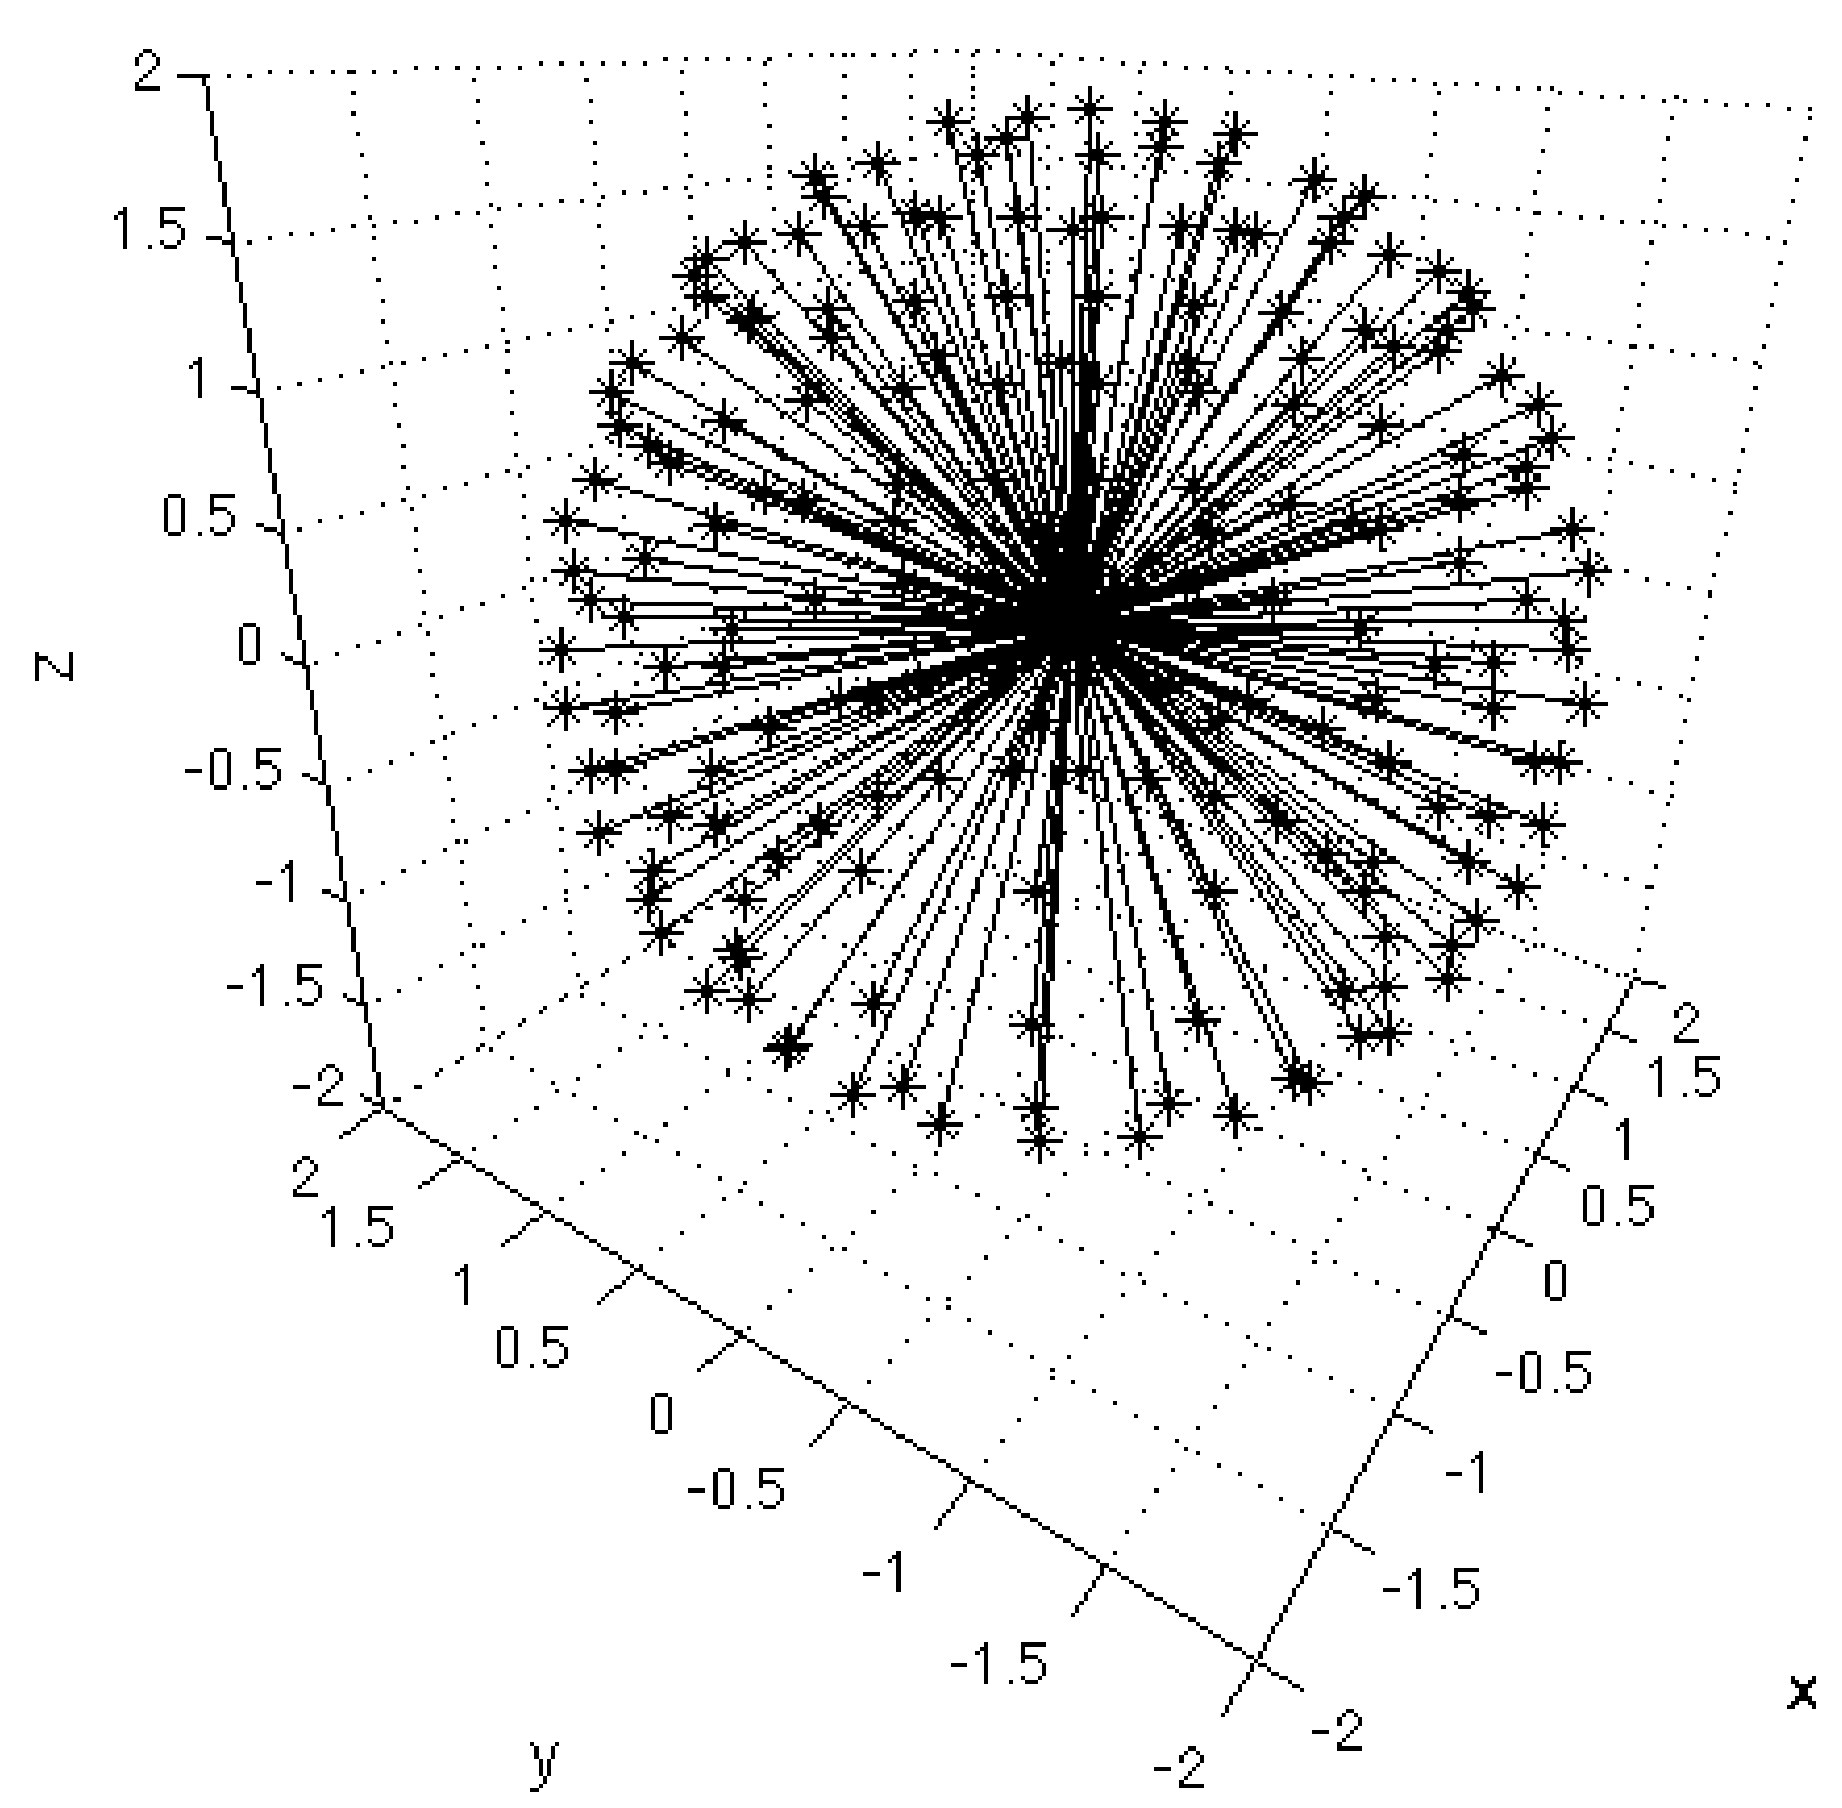
\includegraphics[width=\textwidth]{images/sphere-xyz-01.png}
	\caption{Locations of all 187 Head Related Impulse Responses relative to the user's head.}
	\label{fig:ircam-listen}
\end{figure}



                
\begin{figure}
        \centering
        \begin{subfigure}[b]{0.49\textwidth}
                \centering
                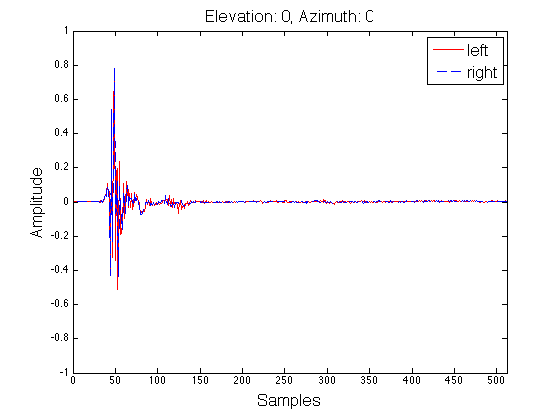
\includegraphics[width=\textwidth]{images/el0-az0.png}
                \caption{Front}
                \label{fig:gull}
        \end{subfigure}%
        \begin{subfigure}[b]{0.49\textwidth}
                \centering
                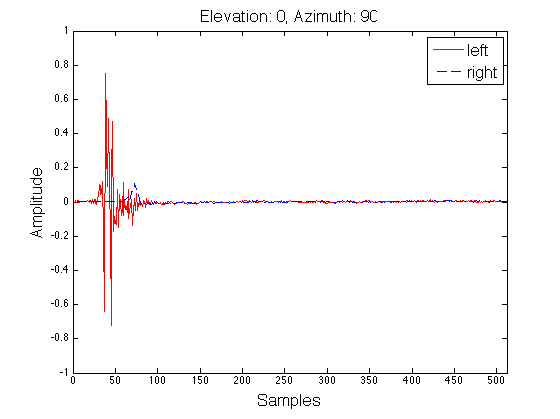
\includegraphics[width=\textwidth]{images/el0-az90.png}
                \caption{Left}
                \label{fig:tiger}
        \end{subfigure}
        \begin{subfigure}[b]{0.49\textwidth}
                \centering
                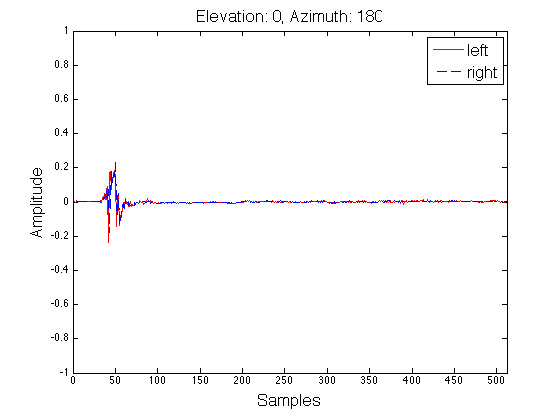
\includegraphics[width=\textwidth]{images/el0-az180.png}
                \caption{Behind}
                \label{fig:mouse}
        \end{subfigure}
        \begin{subfigure}[b]{0.49\textwidth}
                \centering
                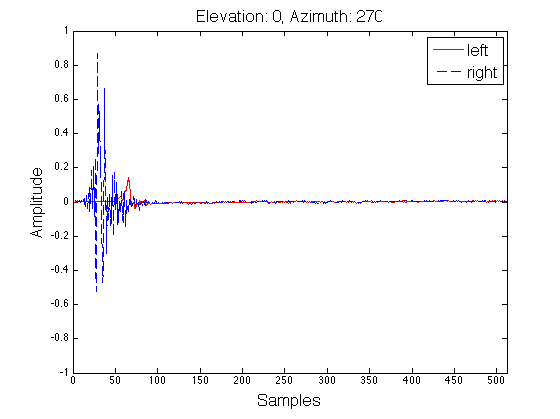
\includegraphics[width=\textwidth]{images/el0-az270.png}
                \caption{Right}
                \label{fig:mouse}
        \end{subfigure}
        \caption{Example signals for the Head Related Impulse Responses of 4 different positions.}\label{fig:ircam-hrir}
\end{figure}

The IRCAM LISTEN database comes with 71 sets of 187 recordings, where each set comes from a different participant, and thus has slightly different responses (due to the individual features of their head, such as the shape of their ear or nose) .  Each recording is 8192 samples long at 44100 Hz sample rate.  Figure \ref{fig:ircam-listen} depicts the locations of all the ``clicks'' in relation to the user's head while Figure \ref{fig:ircam-hrir} depicts 4 filters from a single individual's recordings, IRCAM 1087, from an elevation equal to the individual's ears and placed to the front, left, back, and right of the center of the head at a distance of 1.95 meters away.  Using all 187 recordings gives a reasonable sampling of the space around a user's head, creating a set of ITL's with known relative locations.  Thus, any sound can be binauralized by using any of the 187 recordings.  However, as these are all spaced at 1.95 meters away from the user's head, a sound that is closer or farther away than 1.95 meters must be attenuated.  Further, these 187 sampled locations must be converted to a continuous sampling, allowing for a sound to be binauralized anywhere on surface of a sphere, through the use of interpolation.  To achieve both of these extra features, I use a k-Nearest Neighbor tree using the 3 closest neighbors to a point on a sphere.  These three nearest points are then averaged to produce the final left and right ear filters.  The average distance to the nearest filters are used to attenuate the final filter using a logarithmic relationship between distance and attenuation, simulating the logarithmic perception of sound (decibels).

Any incoming sound may then be filtered using the final combined and attenuated filter.  To filter the original sound with the binaural filters, we make use of an FFT-based convolution to filter the original sound with the binaural filters.  We first remove most of the silence from all filters, cropping the original 8192 sample filters to 512 samples.  Then, an incoming sound wave is chunked in 512 sample frames.  The resulting convolution of the original frame and the filter is $(2N + 1)$ samples long. To achieve continuous filtering, we use an overlap-add operation.  Overlap-add takes the additional resonance, or the additional 513 samples as a result of the convolution operation, and adds this as an overlapping part to the next frame of filtering.  This ensures any energy in the system is continuously kept in the filtering procedure.  

\subsubsection{GPS}

A user's location is obtained using Apple's CoreLocation framework.  This provides a latitude, longitude, and altitude using Global Positioning System (GPS).  As this defines a point on a Earth through a spherical coordinate system, this location must be converted to a 3-dimensional cartesian point to be used with the filter tree in Figure \ref{fig:ircam-listen}.  For this purpose, a specific projection which flattens the Earth's surface to a 2-dimensional landscape must be used.  We make use of the Universal Transverse Mercator (UTM) coordinate system which maps latitude and longitude locations to a mercator projection, and is described in detail in the 330-page document, Bulletin 1532, by the United States Geological Survey \cite{}.  Any new ``graffiti'' is then given the user's current UTM $x,y$ and altitude.  

CoreLocation also provides different modes of accuracy depending on the application's needs.  As ``Sonic Graffiti'' requires a high precision of accuracy, this was set to ``kCLLocationAccuracyBestForNavigation'', which the Apple Developer Documentation\footnote{\url{https://developer.apple.com/library/mac/documentation/CoreLocation/Reference/CoreLocationConstantsRef/Reference/reference.html#//apple\_ref/c/data/kCLLocationAccuracyBest}} describes as:

\begin{quotation}
Use the highest possible accuracy and combine it with additional sensor data. This level of accuracy is intended for use in navigation applications that require precise position information at all times and are intended to be used only while the device is plugged in.
\end{quotation}

During the development of this application, it was found that accuracy when not moving was unreliable to at least 10 meters.  When moving, however, particularly in a straight line, accuracy was more reliable, perhaps to within 1 meter.  As an example, the plots in Figure \ref{fig:gps-tracking} show two example paths taken by me walking around a single block in London.  

\subsubsection{Sonification}

The resulting sonification of any recorded graffiti is achieved through (1) discovering the relative position of the graffiti to the user's current location and orientation, (2) binauralizing the individual graffiti using the procedure described in Section \ref{sec:binauralization}, resulting in a stereo audio signal, (3), summing all resulting binauralizations, and (4) mixing the resulting stereo sum using a compressor so that the signal is within the speaker's limits.   

During initial tests, only 2 - 3 sounds could be binauralized at a time, before clicks and buffer underruns occurred.  These are typical signs that a CPU cannot keep up with processing and is instead opting out of processing audio for a few frames until processing can catch up.  

\subsubsection{Vectorization}

In order to increase the number of sounds that could be binauralized without CPU lags, we made use of vector-based acceleration.  This is a technique that takes advantage of large register sizes in CPU architecture, in this case 16-bytes.  Instead of performing an operation on a single byte, or in the case of floating-point data, 4 bytes, the same operation may be performed on 16-bytes using larger registers.  Further, if the amount of memory is fixed to a certain size, for-loops which require branching on each iteration may be sacrificed through the use of larger register operations, requiring far less branches.  These optimizations are cleverly implemented in the Apple Accelerate Framework, making many arithmetic operations very fast to perform.  After rewriting the binauralization routines in Accelerate language, I could binauralize 25-30 sound sources before clicks and buffer underruns occurred. 

\subsection{GUI}

\subsection{Discussion}

Sonic Graffiti allows a user to record a sound based on the current GPS location of the device.  The resulting sound is played back as a continuous loop and spatialized based on the user's relative location to the original recorded location.  This is achieved through the use of a bespoke binauralization library.  As the routines require significant processing as the number of sounds increase, vectorization was used to accelerate computation.  The resulting framework has been made available online for anyone to use at \url{http://github.com/pkmital}.

\section{Future Echoes}

Next are two installation outputs developed as part of a course I led in a design school in India which explore the use of cut-up technique in delivering a spatialized sonic narrative and the use of sound input as a target for a video-based triptych collage.  

\subsection{Ambisonics}


\section{Infected Puppets}


\section{Memory Mosaic}


The juxtaposition of fragments of sound as an arts practice has roots at least as early as music concrete, a compositional technique assembling various natural found sounds in order to produce a collage of sound.  Digital Sampling came in the 1970's allowing sound segments to be triggered using an interface such as a keyboard or pad.  More recent techniques have focused on corpus-based concatenative synthesis, where a target sound is matched to a stored database of segments or sounds (for a comprehensive review, see \cite{Schwarz2006}).  Our technical framework most closely resembles SoundSpotter \cite{CaseyICMC2007}, as its framework provides the basis of our auditory feature transformation described in Section \ref{subsec:acoustic-scene-description}.  Though, of the previous techniques mentioned including those in the review article, none investigate corpus-based concatenative synthesis as a real-time experience in an augmented reality.

%Before reaching the culmination of my sound-based practice in ``Memory Mosaic'', an iOS application which automatically creates sound collages based on an aggregation of learned sounds, I will discuss a few practice-based outputs that led me to this application.  
%The first application, ``Sonic Graffiti'', grew out of the desire to create a representation of sonic memories as a spatialized global sonic map.  




%\subsection{Sonic Memory}
%Motivation for implementing an augmented reality which stores ``sonic memories'' and resynthesizes them using the incoming input comes from literature investigating  

\section{Machine Listening Model}
\label{sec:machine-listening-model}

The machine listening model employed in Memory Mosaic is motivated by evidence in  literature of auditory perception stressing the importance of temporal regularities of an acoustic scene in providing continuity for maintaining a cognitive model of an acoustic scene (see \cite{Winkler2009a} for a recent in-depth review).  Such research reinforces Bregman's theory of streaming \cite{Bregman1990}, where one phase consists of the formation of primitive based features, and another on the schema-based selection of streams.  Our model thus places emphasis on temporal discontinuities of the auditory stream using a description of the acoustic scene based on the well-known cepstral coefficients.  % All math operations, including FFT, addition, subtraction, and multiplication are performed using the Apple Accelerate framework in order to achieve real-time performance on an iPhone.  These libraries are made freely available by the authors here: \url{http://github.com/pkmital}.

\subsection{Acoustic Scene Description}
\label{subsec:acoustic-scene-description}

% this needs expanding
Numerous measures of an acoustic scenes have been investigated ...  We make use of one that has the benefit of describing as much of the structure of the acoustic space as possible in order to investigate the regularities at any spectral bandwidth.  

Details of the Log Frequency Cepstral Coefficients (LFCC) feature transformation are described in \cite{CaseyICMC2007}, though is reiterated here for completeness.  The feature transformation begins with the Fast Fourier Transform (FFT) of an audio signal using a fixed frame-size.  For the purposes of real-time augmented reality on the iPhone, at a sample rate of 44100 Hz, a 4096-sample FFT provides high spectral resolution while still being fast enough to perform in real-time.  Following the real-FFT, the magnitudes undergo a Constant-Q Transform (CQT), a real log base-10 operation, and a Discrete Cosine Transform (DCT) in order to produce the 89-element LFCC feature vector.

\subsection{Segmentation Model}

Discontinuity of the spectral shape of an acoustic scene is determined using a statistical model employing the mean and variation of the differences on the distances to a low-pass signal of the features.  The model is described in the Figure \ref{fig:segmentation-model}.  Following the feature transformation, the model has two states of operation: segmenting or not.  When the model is not segmenting, the model of background is built up until a discontinuity appears.  Similarly, for the foreground model, a separate model of the foreground is built up from the start of the segment.  Aside from detecting the discontinuity within the foreground model, the model also detects if the current frame returns to the background model by computing distance to the background model.  Using a prior assumption of a normally distributed feature-space, <<GET A PLOT OF A BUSY STATION'S DISTRIBUTION OF FEATURE VALUES>> we compute deviations of the background and foreground model past 3 standard deviations.  As well, checking whether the currently observed audio frame returns to background, we check if its features are within 3 standard deviations of the background model and stop segmenting.  A parameter controlling the threshold of the standard deviation, between 0.1 and 3.0 standard deviations, is described in Section \ref{subsec:parameters}.

Each new segment detected is written to disk using Apple's Extended Audio File Format.  Only the audio segment's first frame's 89-dimensional LFCC feature vector is retained in memory in order to form a matrix of vectors.  As our model is based on attentional shifts,

% uhh...

\section{Concatenative Synthesis Engine}

The concatenative synthesis engine describes any input sound using a polyphonic reconstruction from its database of sound segments.  At each new onset determined by a temporal irregularity of the acoustic scene, a new set of matches are constructed to the current audio frame.  The onset detection for the synthesis engine is much like the one for the segmentation model; however, no foreground model is kept, and only the background model may deviate, creating new background models at each onset.  Thus, the model does not require knowing what is foreground or background, and only requires deviations in the continuous acoustic space.  

% include graphic of the algorithm here.  

\subsection{Matching}

Matching can be formulated as a nearest neighbor algorithm which begins by creating a metric space $X$ of known points $P = p_1, p_2, ..., p_n$ for $n$ points.  These points are pre-processed in such a way that a neighbors to any query point, $q \in X$, are found quickly.  To pre-process the points, we use a distance metric to keep the 3 highest matches to any query point using a simple linear index.  Iterating linearly over the dataset of LFCC vectors, the 3 best matched vectors' indices are kept using cosine similarity, which measures the angle between two vectors $A$ and $B$ like so:

\begin{math}
\textnormal{similarity} = \cos(\theta) = {A \cdot B \over |A| |B|} = \frac{ \sum\limits_{i=1}^{n}{A_i \times B_i} }{ \\ \sqrt{\sum\limits_{i=1}^{n}{(A_i)^2}} \times \sqrt{\sum\limits_{i=1}^{n}{(B_i)^2}}} 
\end{math}

Using Apple's Accelerate framework, this metric can be computed using efficient vector operations that are optimized for the iPhone:
\clearpage
\begin{lstlisting}
float cosineDistance(float *x, float *y, unsigned int length) {
	float dotProd, magX, magY;
	float *tmp = (float*)malloc(count * sizeof(float));
	
	vDSP\_dotpr(x, 1, y, 1, &dotProd, length);
	
	vDSP\_vsq(x, 1, tmp, 1, length);
	vDSP\_sve(tmp, 1, &magX, length);
	magX = sqrt(magX);
	
	vDSP\_vsq(y, 1, tmp, 1, length);
	vDSP\_sve(tmp, 1, &magY, length);
	magY = sqrt(magY);
	
	delete tmp;
	
	return 1.0 - (dotProd / (magX * magY));
}
\end{lstlisting}

\section{Application}

\subsection{Parameters}
\label{subsec:parameters}

\section{Discussion}

John Oswald; Burrough's Cut-up-technique; Scrambled Hackz; Collins; Casey; Grierson; Schwarz...